\subsection{Парабола}

\begin{wrapfigure}[8]{r}{0.45\tw}
    \centering
    \vspace{-0.7pc}
    \tikzsetnextfilename{parabola}
    \begin{tikzpicture}
       \def\xmax{2.4}
       \def\k{0.33}
       \def\x{1/(4*\k)}


       \tkzDefPoint(-\xmax,{\xmax*\xmax*\k}){X0}
       \foreach \x in {-2.4,-2.35,...,2.4} {
           \def\y{\x*\x*\k}
           \tkzDefPoint(\x,\y){X1}
           \tkzDrawSegment[thick](X0,X1)
           \tkzDefShiftPoint[X1](0,0){X0}
       }

       \tkzDefPoint(0,0){O}
       \tkzDefPoint(0,{1/(4 *\k)}){F}
       \tkzDefPointBy[homothety=center O ratio -1](F) \tkzGetPoint{D}
       \tkzDefPointBy[homothety=center O ratio 2](F) \tkzGetPoint{F'}
       \tkzDefPointWith[orthogonal,K={2*\k *\xmax}](D,F) \tkzGetPoint{D1}
       \tkzDefPointBy[homothety=center D ratio -1](D1) \tkzGetPoint{D2}

       \tkzDefPointWith[orthogonal,K=-1](F,D) \tkzGetPoint{P}
       \tkzDefPointBy[projection = onto D1--D2](P)  \tkzGetPoint{P'}

       \tkzDefPoint(-\x, \k*\x*\x){X}
       \tkzDefPointBy[projection = onto D1--D2](X)  \tkzGetPoint{X'}

       \tkzMarkRightAngles[size=0.2](D2,D,F F',F,P D,P',P D2,X',X)


       \tkzDrawSegments[semithick](D1,D2 F,P P,P' F,X X,X')

       \tkzDrawSegment[dim={{$q$},{\xmax*0.9},right=1mm, midway}](F,O)
       \tkzDrawSegment[dim={{$q$},{\xmax*0.9},right=1mm, midway}](O,D)

       \tkzLabelPoint[above right=-1pt](F){$\mathbf{F}$}
       \tkzLabelPoint[below right=-2pt](O){$\mathbf{O}$}
       \tkzLabelPoint[below left=-2pt](X){$\mathbf{X}$}
       \tkzLabelSegment[above](F,P){$p$}
       \tkzLabelSegment[left](P,P'){$p$}
       \tkzLabelSegment[above left=-4pt](F,X){$r$}
       \tkzLabelSegment[right](X,X'){$d$}

       \tkzDrawSegments[dash dot, semithick](D,F')
       \tkzDrawSegments[semithick](D,F)

       \tkzDrawPoints(O, F, P, X)
        
    \end{tikzpicture}
    \caption{Парабола}
    \label{pic:parabola}
\end{wrapfigure}
\term{Парабола}~--- геометрическое место точек, равноудалённых от заданной прямой~--- \term{директрисы} параболы, и заданной точки~--- \term{фокуса} параболы.

Получим из определения параболы её уравнение в декартовых координатах. Пусть расстояние между фокусом и директрисой параболы равно $p$. Из определения ясно, что существует точка параболы $P$, располагающаяся в середине перпендикуляра, опущенного из фокуса на директрису. Расположим параболу так, чтобы эта точка оказалась в начале координат, директриса задавалась уравнением $x = -p/2$, а фокус имел координаты $(p/2, 0)$.

Приравняем расстояния от произвольной точки параболы с координатами $(x, y)$ до директрисы и до фокуса:
\begin{gather*}
    x + \frac{p}{2} = \sqrt{\left(x - \frac{p}{2} \right)^2 + y^2},\\
    x^2 + \frac{p^2}{4} + px = x^2 + \frac{p^2}{4} - px + y^2,\\
    y^2 = 2px. \tag{\theequation}
\end{gather*}

Полученное равенство является каноническим уравнением параболы в декартовых координатах. В силу симметрии данного уравнения, перпендикуляр, опущенный из фокуса на директрису, является \imp{осью} параболы, а точка $P$~--- её \imp{вершиной}.

Легко заметить, что длина перпендикуляра, опущенного из фокуса на параболу, равна $p$. Этот отрезок называется \term{фокальным параметром}, а его длина, как следует из вышесказанного, равна расстоянию от фокуса до директрисы.

\begin{wrapfigure}[9]{r}{0.4\tw}
    \centering
    \vspace{-1pc}
    \tikzsetnextfilename{parabola-polar-coord}
    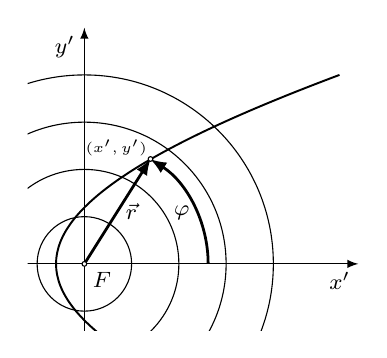
\begin{tikzpicture}[scale=1.2]
        \footnotesize
        \clip (-.3, -0.7) rectangle + (3.5, 3.2);

        \coordinate (xy) at (1, 1.11) {};
        \coordinate (F) at (.3, 0) {};

        \draw [line width = .7pt](3, 2) .. controls (-1, .5) and (-1, -.5) .. (3, -2);

        \draw [-latex] (.3, -2.2) -- (.3, 2.5);
        \draw [-latex] (-1, 0) -- (3.2, 0);

        \draw (F) circle (.5);
        \draw (F) circle (1);
        \draw (F) circle (1.5);
        \draw (F) circle (2);
        \draw (1.61, 0) [-latex, line width=1pt] arc (0:57.8:1.31);
        \draw [-latex, line width=1pt] (.3, 0) -- (1, 1.11);

        \draw (1.05, 1.05) node [anchor=south east] {\tiny{$(x', y')$}};
        \draw (F) node [anchor=north west] {$F$};
        \draw (.65, .55) node [anchor=west] {$\vec r$};
        \draw (1.5, .7) node [anchor=north east] {$\boldsymbol{\varphi}$};
        \draw (3.2, 0) node [anchor=north east] {$x'$};
        \draw (-.1, 2.5) node [anchor=north west] {$y'$};

        \draw (F) [fill=white] circle(.025);
        \draw (xy) [fill=white] circle(.025);
    \end{tikzpicture}
    \caption{}
    \label{pic:parabola-polar-coord}
\end{wrapfigure}
Перенесем теперь фокус параболы в начало координат и получим уравнение параболы в полярных координатах. Для этого нужно сделать такую замену: $x' \hookrightarrow x - p/2$, значит $x \hookrightarrow x' + p/2$, а $y' \hookrightarrow y$. Запишем уравнение параболы в новых координатах:
\begin{gather*}
    y^2 = 2px,\\
    (y')^2 = 2 p \left(x' + \frac{p}{2} \right).
\end{gather*}
Перейдём в полярные координаты в полученном равенстве:
\begin{gather*}
    r^2 \sin^2 \varphi = p^2 + 2pr\cos \varphi,\\
    r^2 \cdot \sin^2 \varphi - r \cdot 2 p  \cos \varphi - p^2,\\
    D = 4p^2 \cos^2 \varphi + 4 p^2 \sin^2 \varphi = 4 p^2,\\
    r = \frac{2p \cos \varphi \pm 2p}{2\sin^2 \varphi}, \quad r \geqslant 0,\\
    r = \frac{p (\cos \varphi + 1)}{1 - \cos^2 \varphi} = \frac{p (\cos \varphi + 1)}{(1 - \cos\varphi)(1 + \cos\varphi)} = \frac{p}{1 - \cos \varphi}.
\end{gather*}
Если же параболу развернуть на $180^\circ$, в знаменателе будет знак плюс. Это завершает вывод уравнения параболы в полярных координатах:
\begin{equation}
    r = \frac{p}{1 \pm \cos \varphi}.
\end{equation}

\begin{wrapfigure}{r}{0.45\tw}
    \centering
    \vspace{-.5pc}
    \tikzsetnextfilename{parabola-optic-property}
    \begin{tikzpicture}[scale=1.2]
        \footnotesize
        \clip (-.4, -1) rectangle + (4, 3.5);

        \coordinate (xy) at (1, 1.11) {};
        \coordinate (F) at (.3, 0) {};

        \draw [line width = .7pt](3, 2) .. controls (-1, .5) and (-1, -.5) .. (3, -2);

        \draw [-latex] (0, -2.2) -- (0, 2.5);
        \draw [-latex] (-1, 0) -- (3.5, 0);

        \draw [-latex, line width=1pt] (F) -- (xy);
        \draw [-latex, line width=1pt] (xy) -- (2, 1.11);
        \draw [-latex, line width=1pt] (xy) -- (2, 1.67);
        \draw (xy) -- (3, 1.11);
        \draw [dashes] (3, 2.21) -- (-.5, 0.29);

        \draw (1.2, 1.11) node [anchor=south east] {$(x, y)$};
        \draw (F) node [anchor=north] {$F$};
        \draw (.65, .55) node [anchor=west] {$\vec r$};
        \draw (1.5, 1.11) node [anchor=north] {$\vec x$};
        \draw (1.5, 1.39) node [anchor=south] {$\vec t$};

        \draw (3.5, 0) node [anchor=north east] {$x$};
        \draw (0, 2.5) node [anchor=north west] {$y$};

        \draw (F) [fill=white] circle(.025);
        \draw (xy) [fill=white] circle(.025);
    \end{tikzpicture}
    \caption{}
    \label{pic:parabola-optic-property}
\end{wrapfigure}
Как и все конические сечения, парабола обладает \imp{оптическим свойством}, которое формулируется таким образом: пучок лучей, параллельных оси параболы, отражаясь в последней, собирается в её фокусе. И наоборот, свет от точечного источника, находящегося в фокусе, отражается параболой в пучок параллельных её оси лучей.

Аналогично доказательству оптического свойства эллипса рассмотрим случай только верхней ветви. Выберем на ней произвольную точку $(x, y)$. Тогда вектор, определяющий направление луча из фокуса в выбранную точку задается вектором $\vec r = (x - p/2, y)$. Направление, соответствующее оси параболы, зададим единичным вектором $\vec x = (1, 0)$, так как ось параболы с каноническим уравнением совпадает с осью абсцисс. Остается найти вектор $\vec t$ касательной в точке $(x, y)$. Для верхней ветви параболы каноническое уравнение эквивалентно $y = \sqrt{2px}$. Найдем производную данной функции:
\begin{gather*}
    y' = \frac{2p}{2\sqrt{2px}} = \sqrt{\frac{p}{2x}}.
\end{gather*}
Значит направляющий вектор касательной можно представить в виде
\begin{equation*}
    \vec t =
    \begin{pmatrix}
        1\\
        y'_x
    \end{pmatrix} =
    \begin{pmatrix}
        1\\
        \sqrt{\dfrac{p}{2x}}
    \end{pmatrix}.
\end{equation*}

Остается проверить равенство косинусов углов между векторами $\vec r$ и $\vec t$ и векторами $\vec x$ и $\vec t$:
\begin{gather*}
    \frac{\scalar{r}{t}}{|\vec r| | \vec t|} = \frac{\scalar{x}{t}}{|\vec x| |\vec t|},\\
    \scalar{r}{t} = |\vec r| \scalar{x}{t},\\
    \left(x - \frac{p}{2}\right)\cdot 1 + y \cdot \sqrt{\frac{p}{2x}}  = \sqrt{\left( x - \frac{p}{2} \right)^2 + y^2 } \left(1 \cdot 1 + 0 \cdot \sqrt{\frac{p}{2x}} \,\right),\\
    \left(x - \frac{p}{2}\right)^2 + \frac{y^2 p}{2x} + 2 y \sqrt{\frac{p}{2x}} \left(x - \frac{p}{2}\right) = \left(x - \frac{p}{2}\right)^2 + y^2,\\
    2  \sqrt{\frac{p}{2x}} \left(x - \frac{p}{2}\right) =  y \left( 1 - \frac{p}{2x} \right),\\
    \sqrt{\frac{4x^2p}{2x}} \left(1 - \frac{p}{2x}\right) =  y \left( 1 - \frac{p}{2x} \right),\\
    \sqrt{2xp}  =  y.
\end{gather*}
Получено уравнение верхней ветви параболы, которому, очевидно, координаты точки, принадлежащей параболе, удовлетворяют. Следовательно, оптическое свойство доказано.

Покажем, что парабола является коническим сечением. Для этого рассмотрим каноническое уравнение конической поверхности
\begin{equation*}
    \frac{x^2}{a^2} + \frac{y^2}{b^2} - \frac{z^2}{c^2} = 0
\end{equation*}
и секущую плоскость, параллельную образующей конуса и задаваемую уравнением
\begin{equation*}
    z = \frac{c(x + d)}{a},
\end{equation*}
где коэффициенты $a, b, c$ определяют вид поверхности, а $d$~--- положение плоскости. Подставим второе в первое:
\begin{gather*}
    \frac{x^2}{a^2} + \frac{y^2}{b^2} = \frac{x^2 + d^2 + 2yd}{a^2},\\
    \frac{y^2}{b^2} = \frac{d^2 + 2xd}{a^2},\\
    y^2 = 2 x \underbrace{\frac{b^2d}{a^2}}_p + \frac{b^2 d^2}{a^2}.
\end{gather*}
С точностью до вертикального сдвига получено каноническое уравнение параболы, что подтверждает принадлежность параболы множеству конических сечений.

